\documentclass[8pt,a4paper,twoside]{article}

% Basic packages
\usepackage{amsmath, amssymb}
\usepackage{graphicx}
\usepackage{xcolor}
\usepackage[margin=2.5cm]{geometry}
\usepackage{float}
\usepackage{wrapfig}
\usepackage{titlesec}
\usepackage{fancyhdr}
\usepackage{caption}
\usepackage{subcaption}
\usepackage{hyperref}
\usepackage{fontspec}
\usepackage{nomencl}
\usepackage{multicol}
\usepackage{etoolbox}
\usepackage{multirow}
\usepackage{csquotes}
\usepackage{tcolorbox}
\usepackage{listings}
\usepackage{booktabs}
\usepackage{enumitem}
\setlist[itemize]{itemsep=2pt, topsep=4pt, parsep=0pt, partopsep=0pt}


% Restore \underbar and \underline before loading sectsty
\let\oldunderbar\underbar
\let\oldunderline\underline
\usepackage{sectsty} % Custom section styles

% Fonts
\setmainfont{Poppins} % Main font
\newfontfamily\titlesfont{Anonymous Pro} % Titles font
\setmonofont{Anonymous Pro} % Monospace font

% Bibliography
\usepackage[backend=biber, style=ieee, citestyle=numeric]{biblatex}
\addbibresource{references.bib}

% Define colors
\definecolor{cherenkovblue}{RGB}{55, 139, 230} % Signature blue
\definecolor{darkgreen}{RGB}{34,139,34}  % Comments (green)
\definecolor{darkorange}{RGB}{255,140,0} % Strings (orange)
\definecolor{blue}{RGB}{30,144,255}      % Keywords (blue)
\definecolor{lightgray}{RGB}{245,245,245} % Background


% Itemize lists use bullets
\renewcommand{\labelitemi}{\textbullet}

% Adjust default font sizes
\renewcommand{\normalsize}{\fontsize{8}{10}\selectfont}
\renewcommand{\small}{\fontsize{7}{9}\selectfont}
\renewcommand{\footnotesize}{\fontsize{7}{9}\selectfont}
% Set caption font size
\captionsetup{
    font=small,
    labelfont=bf,
    textfont=it
}

% Section formatting
\makeatletter
\renewcommand{\section}{\@startsection {section}{1}{\z@}%
  {-3.5ex \@plus -1ex \@minus -.2ex}%
  {2.3ex \@plus.2ex}%
  {\titlesfont\fontsize{14}{16}\bfseries\color{cherenkovblue}\MakeUppercase}}
\makeatother

\subsectionfont{\titlesfont\fontsize{12}{14}\bfseries\color{cherenkovblue}}

% Customize spacing
\setlength{\parskip}{6pt}
\setlength{\parindent}{0pt}
\setlength{\itemsep}{2pt}

% Fancy headers & footers
\fancypagestyle{plain}{\fancyhf{}} % Default plain style
\fancypagestyle{post-index}{
    \fancyhf{}
    \fancyhead[LE]{\textit{Alessandro Borgonovo, Gaia Larici, Riccardo Monti, Simone Pagliuca, Riccardo Ronchi}}
    \fancyhead[RO]{\textit{Integration of Nuclear and Renewable Energy for Carbon Neutral Scenarios}}
    \fancyfoot[LE,RO]{\thepage}
    \renewcommand{\headrulewidth}{0.4pt}
    \renewcommand{\footrulewidth}{0.4pt}
    \setlength{\headheight}{14pt}
}

% Code Formatting
\lstdefinestyle{custombox}{
    backgroundcolor=\color{gray!10},
    frame=single,
    rulecolor=\color{black},
    basicstyle=\ttfamily\small, % Monospace font
    breaklines=true,
    captionpos=b,
    numbers=left,
    numberstyle=\tiny\color{gray},
    keywordstyle=\color{blue}\bfseries,  % Bold blue keywords
    commentstyle=\color{darkgreen}\itshape, % Italic green comments
    stringstyle=\color{darkorange}, % Orange strings
    showstringspaces=false,
    tabsize=4
}
\lstset{style=custombox}

% Define Modelica language
\lstdefinelanguage{Modelica}{
  morekeywords={
    model, equation, end, function, input, output, algorithm, if, then, else, elseif, for, while, loop, when, connect, parameter, constant, discrete, initial, final, public, protected, encapsulated, extends, redeclare, replaceable, inner, outer, import, from, class, record, type, operator, pure, impure, partial, block, connector, expandable, annotation, assert, terminal
  },
  morecomment=[l]{//},
  morecomment=[s]{/*}{*/},
  morestring=[b]",
  morestring=[b]{'}
}

% Box styles
\tcbset{
    boxstyle/.style={
        colframe=cherenkovblue,
        colback=white,
        coltitle=white,
        fonttitle=\bfseries,
        rounded corners,
        width=\textwidth,
        boxrule=0.75mm,
        arc=2mm,
        toptitle=2mm,
        bottomtitle=2mm,
        sharp corners=downhill
    }
}

% Document begins
\begin{document}

% Title Page
\thispagestyle{plain}

% Title with Titles Font (Anonymous Pro)
{\titlesfont\fontsize{18}{22}\textbf{\color{cherenkovblue}{Decarbonizing Sette Laghi \\ Technical, Economic, and Environmental Study}}}\\
{\titlesfont\fontsize{11}{13}\color{cherenkovblue} Politecnico di Milano}\\

\vspace{-8pt}

% Author information with Main Font (Poppins)
{\normalsize\textbf{Alessandro Borgonovo, Gaia Larici, Riccardo Monti, Simone Pagliuca, Riccardo Ronchi}} \\
{\footnotesize\textit{borgo, gaia, riccardo, 10698534, richard}} \\

\vspace{8pt}

% Course and Academic Year
{\footnotesize\textbf{Course:} Integration of Nuclear and Renewables for Carbon Neutral Scenarios}\\
{\footnotesize\textbf{Academic Year:} 2024/2025}\\

% Horizontal rule
\vspace{6pt}
\centerline{\rule{0.95\textwidth}{0.5pt}}
\vspace{8pt}

% Abstract with Titles Font for Heading, Main Font for Body
{\titlesfont\fontsize{10}{12}\textbf{\color{cherenkovblue} ABSTRACT}} 

\vspace{4pt}
{\normalsize
This study evaluates the technical and economic feasibility of integrating Small Modular Reactors (SMRs) into the residential energy sector of the north-western province of Varese, Italy. The proposed hybrid system combines nuclear power with renewable energy sources, hydrogen production, and synthetic methane generation to meet regional energy demands and support decarbonization efforts. The analysis includes dynamic simulations of the plant's operation, economic assessments, and environmental impact evaluations over a 60-year period. The methodology involves data collection from regional energy databases, dynamic modeling using Dymola software, and economic analysis considering capital and operational expenditures, as well as revenue streams from electricity, hydrogen, and synthetic gas sales. Preliminary results indicate the potential for significant decarbonization and energy stability, although further analysis is required to determine the economic viability and optimal configuration of the system. [Placeholder for conclusions: The study concludes with insights into the overall feasibility and potential improvements for the proposed hybrid energy system.]
}

\vspace{10pt}

% Key-words box with Titles Font
\begin{tcolorbox}[arc=0pt, boxrule=0pt, colback=cherenkovblue!60, width=\textwidth, colupper=white]
    {\titlesfont\fontsize{10}{12}\textbf{Key-words:}} Small Modular Reactors (SMRs), Hybrid Energy Systems, Decarbonization, Hydrogen Production, Synthetic Methane, Dynamic Simulation, Economic Feasibility, Environmental Impact, Residential Energy Sector, Renewable Energy Integration
\end{tcolorbox}

\vspace{12pt}

% Nomenclature Definitions
\makenomenclature
\renewcommand\nomgroup[1]{%
\item[\bfseries
\ifstrequal{#1}{A}{Type A}{%
\ifstrequal{#1}{B}{Type B \& Misc}{%
}}%
]}

% Neutronics Quantities
\nomenclature[A]{$math$}{Description ($units-of-measurement$)}

% Data & Statistics
\nomenclature[B]{$math$}{Description ($units-of-measurement$)}

% Two-column layout for the nomenclature
\renewcommand{\nompreamble}{\begin{multicols}{2}}
\renewcommand{\nompostamble}{\end{multicols}}

% Render Nomenclature Without Section Break
\vspace{-5pt} % Adjust spacing to fit table
\printnomenclature

\newpage

% Table of Contents
\tableofcontents
\newpage
\pagestyle{post-index}

% Main Content
\graphicspath{{images/}}
\input{content_0.tex}
\input{content_1.tex}
\section{Modelica Plant Modelling}

\subsection{Plant Components}
PRIMA DI TUTTO IL LAYAOUT

\subsubsection{SMR}

\subsubsection{H2 Plant}

\subsubsection{Methanation Reactor Modeling Approach}

The methanation reactor was modeled in \texttt{Modelica} to simulate the conversion of hydrogen (H\textsubscript{2}) and carbon dioxide (CO\textsubscript{2}) into methane (CH\textsubscript{4}) and water (H\textsubscript{2}O) via the Sabatier reaction:
\begin{equation}
\mathrm{CO_2 + 4H_2 \rightarrow CH_4 + 2H_2O} \qquad \Delta H = -165.1\ \text{kJ/mol}
\end{equation}

To approximate the level of CH\textsubscript{4} produced from a given feed, a dimensionless parameter \texttt{conversionEfficiency} was introduced. This factor (default: 0.78) reflects the maximum chemical efficiency of catalytic methanation as reported in Götz et al.~\cite{Gotz2016}. It represents the fraction of the limiting reactant (either CO\textsubscript{2} or H\textsubscript{2}) that is effectively converted to CH\textsubscript{4}, accounting for reactor inefficiencies and incomplete conversion at realistic temperature and pressure conditions.

The molar output flows are then calculated via stoichiometry:
\begin{align*}
\dot{n}_{\mathrm{CH}_4} &= \dot{n}_{\text{lim}} \cdot \texttt{conversionEfficiency} \\
\dot{n}_{\mathrm{H}_2O} &= 2 \cdot \dot{n}_{\mathrm{CH}_4} \\
\dot{n}_{\mathrm{H}_2} &= \dot{n}_{\mathrm{H}_2,\text{in}} - 4 \cdot \dot{n}_{\mathrm{CH}_4} \\
\dot{n}_{\mathrm{CO}_2} &= \dot{n}_{\mathrm{CO}_2,\text{in}} - \dot{n}_{\mathrm{CH}_4}
\end{align*}

\subsubsection{Turbine}

\subsubsection{Other BOP Components}
Control room, buffers etc etc


\subsection{Demand Definition}
To run the model we decided to compute a priori the daily setpoint for:
\begin{itemize}
  \item Turbine load
  \item HTSE load
  \item Steam tap flow
\end{itemize} 
to do so ..
SPIEGA PROCEDIMENTO DA INPUT FOR MODELICA SECTION DI ENERGY_DEMAND
\subsubsection{Dati che diamo in input}
\subsubsection{Rate limiting}

\subsubsection{Clusters}
spiega che famo i clusters + cita che usiamo dei profili di alcuni gioni particolari per vedere rispospta del sistema
\section{Methodology}


\subsection{Demand Definition}
To run the model we decided to compute a priori the daily setpoint for:
\begin{itemize}
  \item Turbine load, limited between $35\%$ and $100\%$ of the maximum load
  \item HTSE load, limited between $60\%$ and $100\%$ of the maximum load
  \item Steam tap flow from the intermediate pressure of the SMR.
\end{itemize} 

We first evaluated the electricity available for the H$_2$ plant, from which we determined the load that the H$_2$ plant can take.

\begin{equation}
  P_{e, \mathrm{available}} = P_{e, \mathrm{SMR}} + P_{\mathrm{turbogas}}(35\%) - P_{e, \mathrm{grid}}
\end{equation}
\begin{equation}
  \mathrm{load}_{H_2} = \left( \frac{P_{e, \mathrm{available}}}{214} + 0.197775 \right) \cdot \frac{1}{N_{\mathrm{HTSE}} \cdot 0.1}
\end{equation}
Where the relationship $\dot{m}_{H_2} = \frac{P_{e, \mathrm{available}}}{214} + 0.197775$ was found by running a sweep simulation of the HTSE model in Dymola.
The mass flow rate of hydrogen produced, $\dot{m}_{H_2}$, is then divided by the nominal mass flow rate produced by one module ($0.1\,\mathrm{kg/s}$) multiplied by the number of modules $N_{\mathrm{HTSE}}$.
This load then had to be clipped for values between $60\%$ and $100\%$, where $60\%$ is the lower operational limit.

Thereafter we estimated the syngas production rate which from the first simulation appeared to be
\subsubsection{Dati che diamo in input}
a
\subsubsection{Rate limiting}
a

\subsubsection{Clusters}
Spiega che facciamo i clusters e cita che usiamo dei profili di alcuni giorni particolari per vedere la risposta del sistema.
\section{Economic Study}

\subsection{Introduction}
spiegazione della questione di 0 tassi di interesse per tipo di progetto (prestito tax free di UE)

\subsection{CAPEX}
capex con fonti + ipotesi decrescita capex 

\subsection{OPEX}
opex con fonti + ipotesi decrescita opex

\subsection{Revenues}
ricavi con fonti + ipotesi crescita/decrescita ricavi e calcolo PUN etc.. 

\subsection{Economic Results: base case}

\subsubsectionn{Sensitivity Analysis}

\subsection{Economic Results: alternative scenarios}
dato che buco finanziario, i primi 15 anni facciamo solo reattore (full electric) per mettere da parte un po' di profitto
quando la possibilità di decarbonizzare il settore dei trasporti è più matura, dopo 15 anni si costruisce l'impianto secondario 
con HTSE, metanatore e turbina a gas. questo permette di guadagnare di più prima e investire più tardi sui componenti secondari.

risultato è uno scenario ibrido con NPV positivo, con 5 anni in meno di operation per ottimizzare il ricambio di HTSE.




\section{Environmental Impact}
The environmental impact of the plant is assessed based on the following indicators: GHG emissions intensity, water usage, and land use.

The assessment is conducted on the optimized operational scenario in which, for the first 20 years, both reactors are dedicated exclusively to electricity production and sale. After year 20, the secondary section of the plant—comprising High Temperature Steam Electrolyzer (HTSE) units and a methanation system coupled with a turbine—is introduced.

As a result, a higher impact on GHG emissions intensity is expected in the early years, primarily due to the exclusive focus on electricity generation.

\subsection{GHG emissions intensity assessment}

\subsubsection{Assumptions and Methodology}
GHG emissions intensity are evaluated considering:

\begin{itemize}
    \item The impact on the regional energy mix (Lombardy), which is expected to be minor.
    \item The impact on the local mix within the Seven Lakes Region, where the plant has a significantly more noticeable influence.
    \item Emissions related to residual fossil fuel demand for building heating.
    \item Emissions from the transportation sector, expected to decrease due to the hydrogen supplied by the plant directly to this sector.
\end{itemize}

\subsubsection{Data Sources}
\paragraph{GHG emissions intensities}
The data for the current (2023) Lombardy energy mix were sourced from Terna, including imported energy shares. GHG emissions intensity per energy source are based on mean values ~\cite{weisser2007guide}. Specifically, solar photovoltaic (PV) was considered for the "Renewable" share, as it is the most prevalent renewable source and the one of major interest for this study.

The values used are:

\begin{table}[H]
    \centering
    \begin{tabular}{lc}
        \toprule
        \textbf{Energy Source} & \textbf{GHG Intensity (gCO$_2$eq/kWh)} \\
        \midrule
        Coal        & 996 \\
        Natural Gas & 550 \\
        Oil         & 780 \\
        Nuclear     & 12 \\
        Renewables  & 56 \\
        \bottomrule
    \end{tabular}
    \caption{GHG emissions intensities by energy source.}
    \label{tab:ghg_intensity_sources}
\end{table}

For nuclear power, other sources support values around 12 $gCO_{2}eq/kWh$ ~\cite{vinoya2024life} and ~\cite{wang2019comparative}.

Equivalent GHG emissions intensity for plant products are:

\begin{table}[H]
    \centering
    \begin{tabular}{lc}
        \toprule
        \textbf{Product} & \textbf{GHG Intensity (gCO$_2$eq/kWh)} \\
        \midrule
        Hydrogen & 19.39 \\
        Syngas   & 72.76 \\
        \bottomrule
    \end{tabular}
    \caption{Equivalent GHG emissions intensity for plant products}
    \label{tab:plant_products_ghg}
\end{table}

Hydrogen carbon intensity assumes electricity for HTSE is fully supplied by the two SMRs and uses its LHV for evaluating the energy equivalent of hydrogen produced. Syngas is produced with that same hydrogen, produced with nuclear-provided electricity. The $CO_2$ is not considered in the GHG intensity of syngas, as it was explained in the economic section.

\paragraph{Energy consumption Data}
The baseline energy data prior to year 0 are derived from current statistics, with total electricity consumption and imports for Lombardy taken from Terna. Values are computed every 15 years to reflect assumed changes in building energy classifications and related energy demands. An exception is made for year 20 to account for the plant's secondary section's commissioning.

A key assumption is that the electricity produced by the proposed plant displaces imported electricity—an economically rational choice. The renewable share varies across scenarios, reflecting the increasing photovoltaic (PV) penetration over time.

\subsubsection{Calculations}
\paragraph{Regional Energy Mix}
The regional impact is assessed in terms of how the plant alters Lombardy's energy mix, which is expected to be minimal due to its limited size (maximum output of 3 TWh/year vs. 65 TWh/year of yearly regional consumption \cite{terna_consumi}). Nevertheless, the impact is more significant in the first 20 years when the plant contributes only electricity.

The regional mix GHG intensity is calculated as:

\begin{equation}
    \left(\frac{gCO2eq}{kWh}\right)_{mix} = \sum_{i} \left( \left(\frac{gCO2eq}{kWh}\right)_{i} \cdot \chi_{i} \right)
\end{equation}

where $i$ indexes each energy source and each energy source's share $\chi_{i}$ is taken into account.


\paragraph{Local Energy Mix}
Using a methodology analogous to the one applied at the regional level, the electricity consumption of the Seven Lakes Region is estimated based on monthly energy balances and photovoltaic production data previously gathered. The local energy mix is reconstructed using three main components: Nuclear, Renewables, and Fossil. The evolution of this mix over time, and its impact on GHG emissions intensity, is evaluated using the previous approach.

\begin{figure}[H]
    \centering
    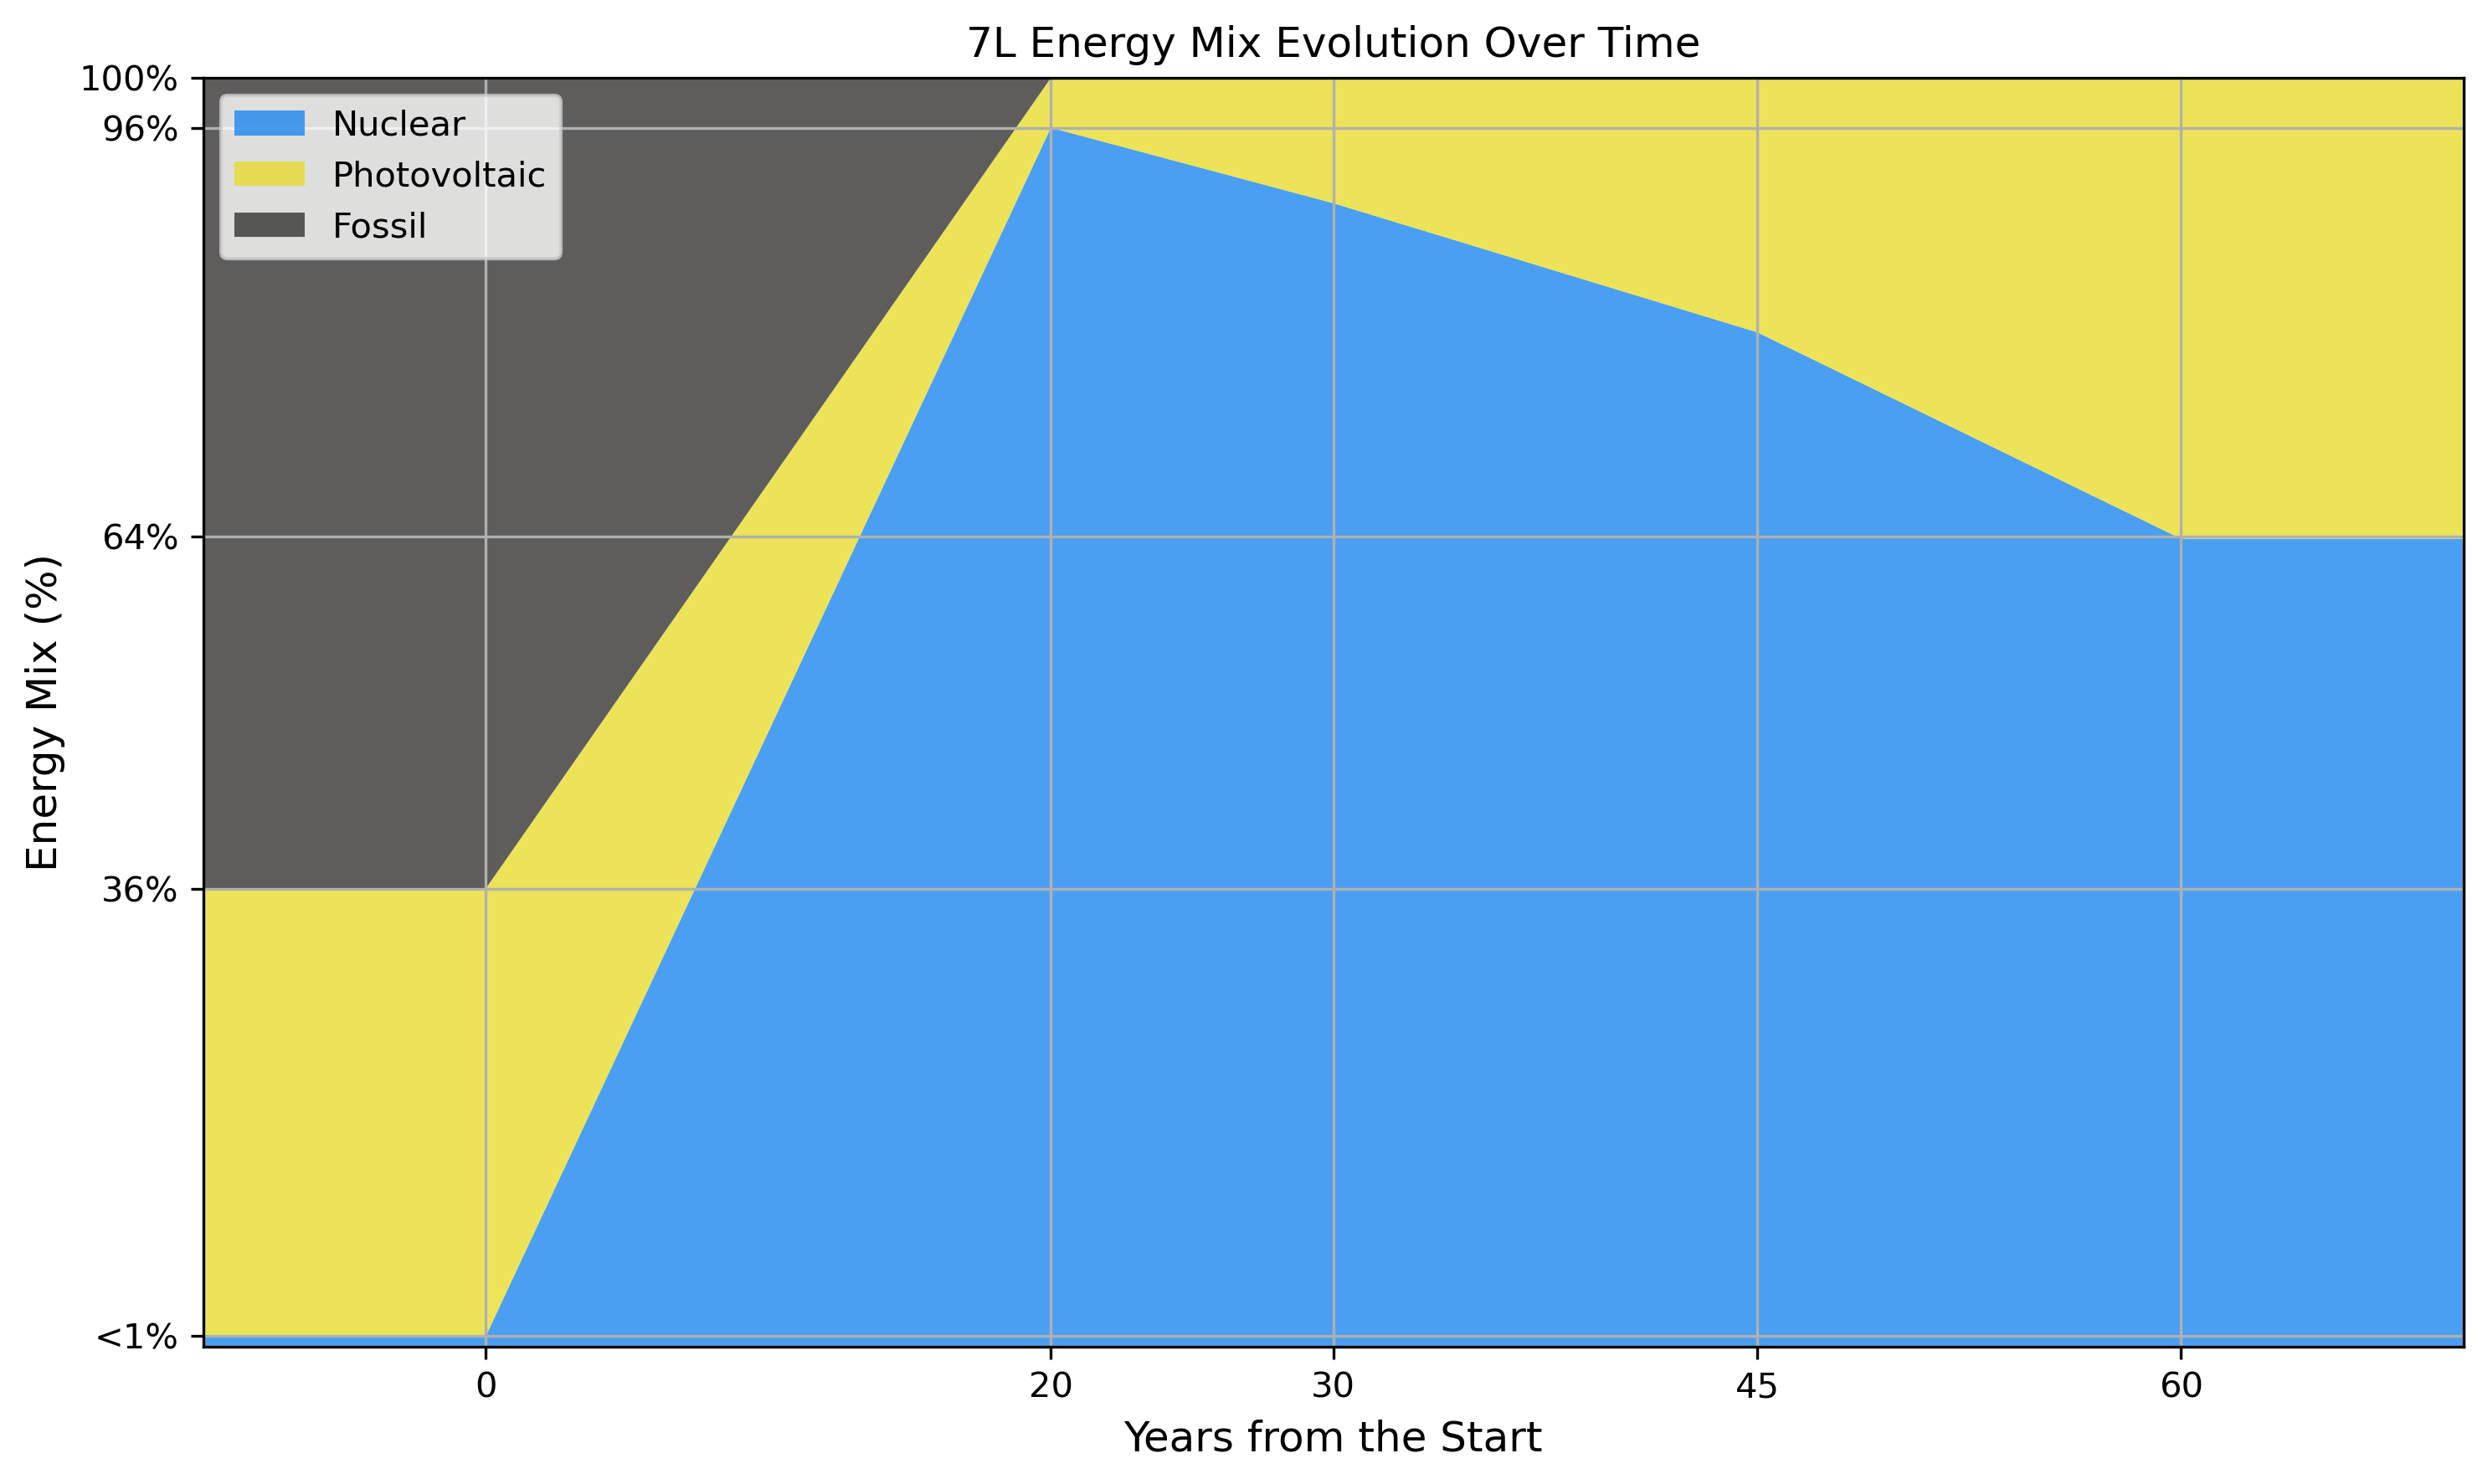
\includegraphics[width=0.8\textwidth]{figures/5_Energy_mix_evolution.png}
    \caption{Local energy mix evolution over time.}
    \label{fig:energy_mix_evolution}
\end{figure}

\paragraph{Residual Fossil Fuel Consumption}
The GHG emissions intensity associated with the residual fossil fuel demand for residential heating are estimated using the processed data, alongside the amount of syngas exported to the market.

The $gCO_{2}eq/kWh$ intensity for this sector is calculated by weighting:
\begin{table}[H]
    \centering
    \begin{tabular}{lc}
        \toprule
        \textbf{Fuel Type} & \textbf{GHG Intensity (gCO$_2$eq/kWh)} \\
        \midrule
        Syngas      & 72.76 \\
        Natural Gas & 550 \\
        \bottomrule
    \end{tabular}
    \caption{GHG intensities for syngas and natural gas in the residential heating sector.}
    \label{tab:residential_heating_ghg}
\end{table}

This impact is zero in the first 20 years of operation, as the plant only provides electricity. From year 21, the introduction of syngas production leads to a growing influence on this sector.

Fossil fuel demand is projected to decrease over time due to improved building energy performance and increased photovoltaic (PV) penetration, while syngas production remains constant — resulting in a gradually increasing contribution to GHG mitigation.


\paragraph{Transportation Sector}
Transport energy consumption data for the region were estimated by scaling national data \cite{eurostat_sankey_2023} according to the population share of the Seven Lakes Region with respect to the national total \cite{istat2023}.

GHG intensities for diesel and gasoline (currently dominant in ground transport) were sourced from \cite{quaschning_co2spec_2025}:
\begin{table}[H]
    \centering
    \begin{tabular}{lcc}
        \toprule
        \textbf{Fuel Type} & \textbf{GHG Intensity (gCO$_2$eq/kWh)} \\
        \midrule
        Diesel    & 266.5 \\
        Gasoline  & 263 \\
        \bottomrule
    \end{tabular}
    \caption{GHG intensities for diesel and gasoline.}
    \label{tab:transportation_ghg}
\end{table}

The impact of the hydrogen produced by the plant is assessed by assuming that it is sold directly to the transportation sector. The resulting GHG intensity is calculated based on the share of energy demand met by:

\begin{table}[H]
    \centering
    \begin{tabular}{lcc}
        \toprule
        \textbf{Energy Carrier} & \textbf{GHG Intensity (gCO$_2$eq/kWh)} \\
        \midrule
        Hydrogen      & 19.39 \\
        Fossil fuels (avg. diesel/gasoline) & 264.75 \\
        \bottomrule
    \end{tabular}
    \caption{GHG intensities for hydrogen and fossil fuels in the transportation sector.}
    \label{tab:transportation_h2_fossil}
\end{table}

Beyond the GHG reduction, it is worth highlighting that hydrogen substitution would also positively affect local air quality due to the elimination of particulate matter emissions typically associated with diesel and gasoline combustion. However, this benefit is not quantified within this study.

\subsubsection{Results}
All results are summarized in the following plots, which illustrate the evolution of GHG emission intensities over time, along with changes in electricity and fossil fuel demand.

\begin{figure}[H]
    \centering
    \begin{minipage}{0.6\textwidth}
        \centering
        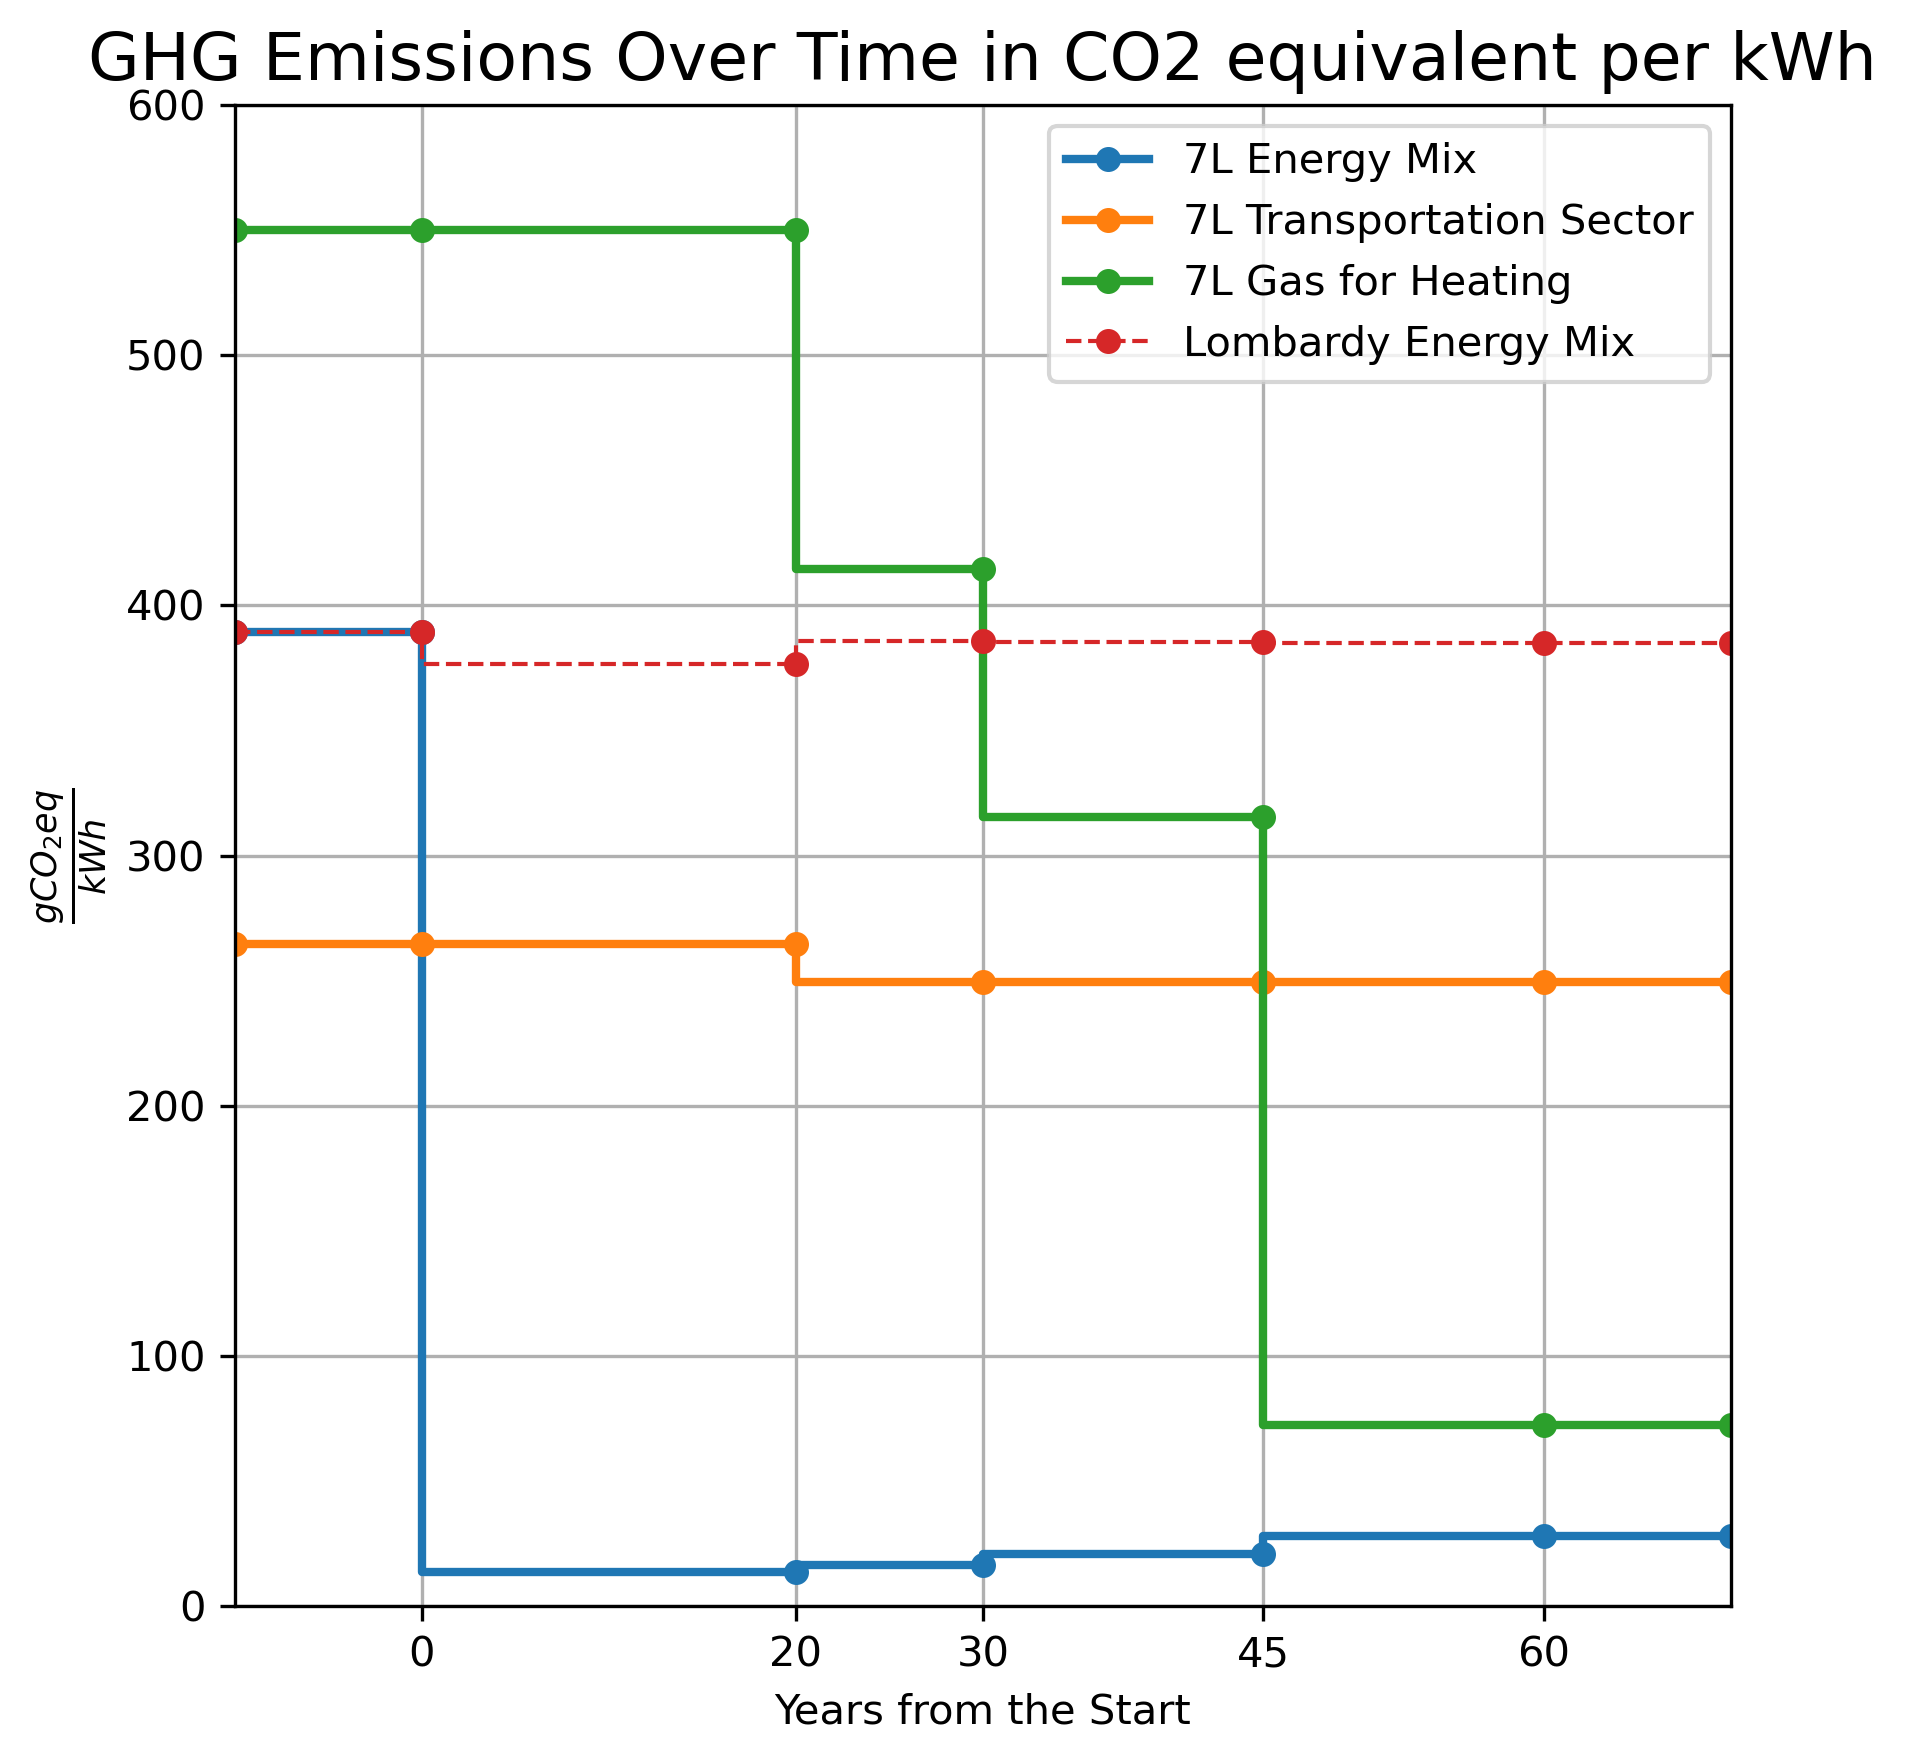
\includegraphics[width=\textwidth]{figures/5_GHG_emissions_over_time.png}
        \caption{GHG emissions intensity over time.}
        \label{fig:ghg_emissions}
    \end{minipage}\hfill
    \begin{minipage}{0.6\textwidth}
        \centering
        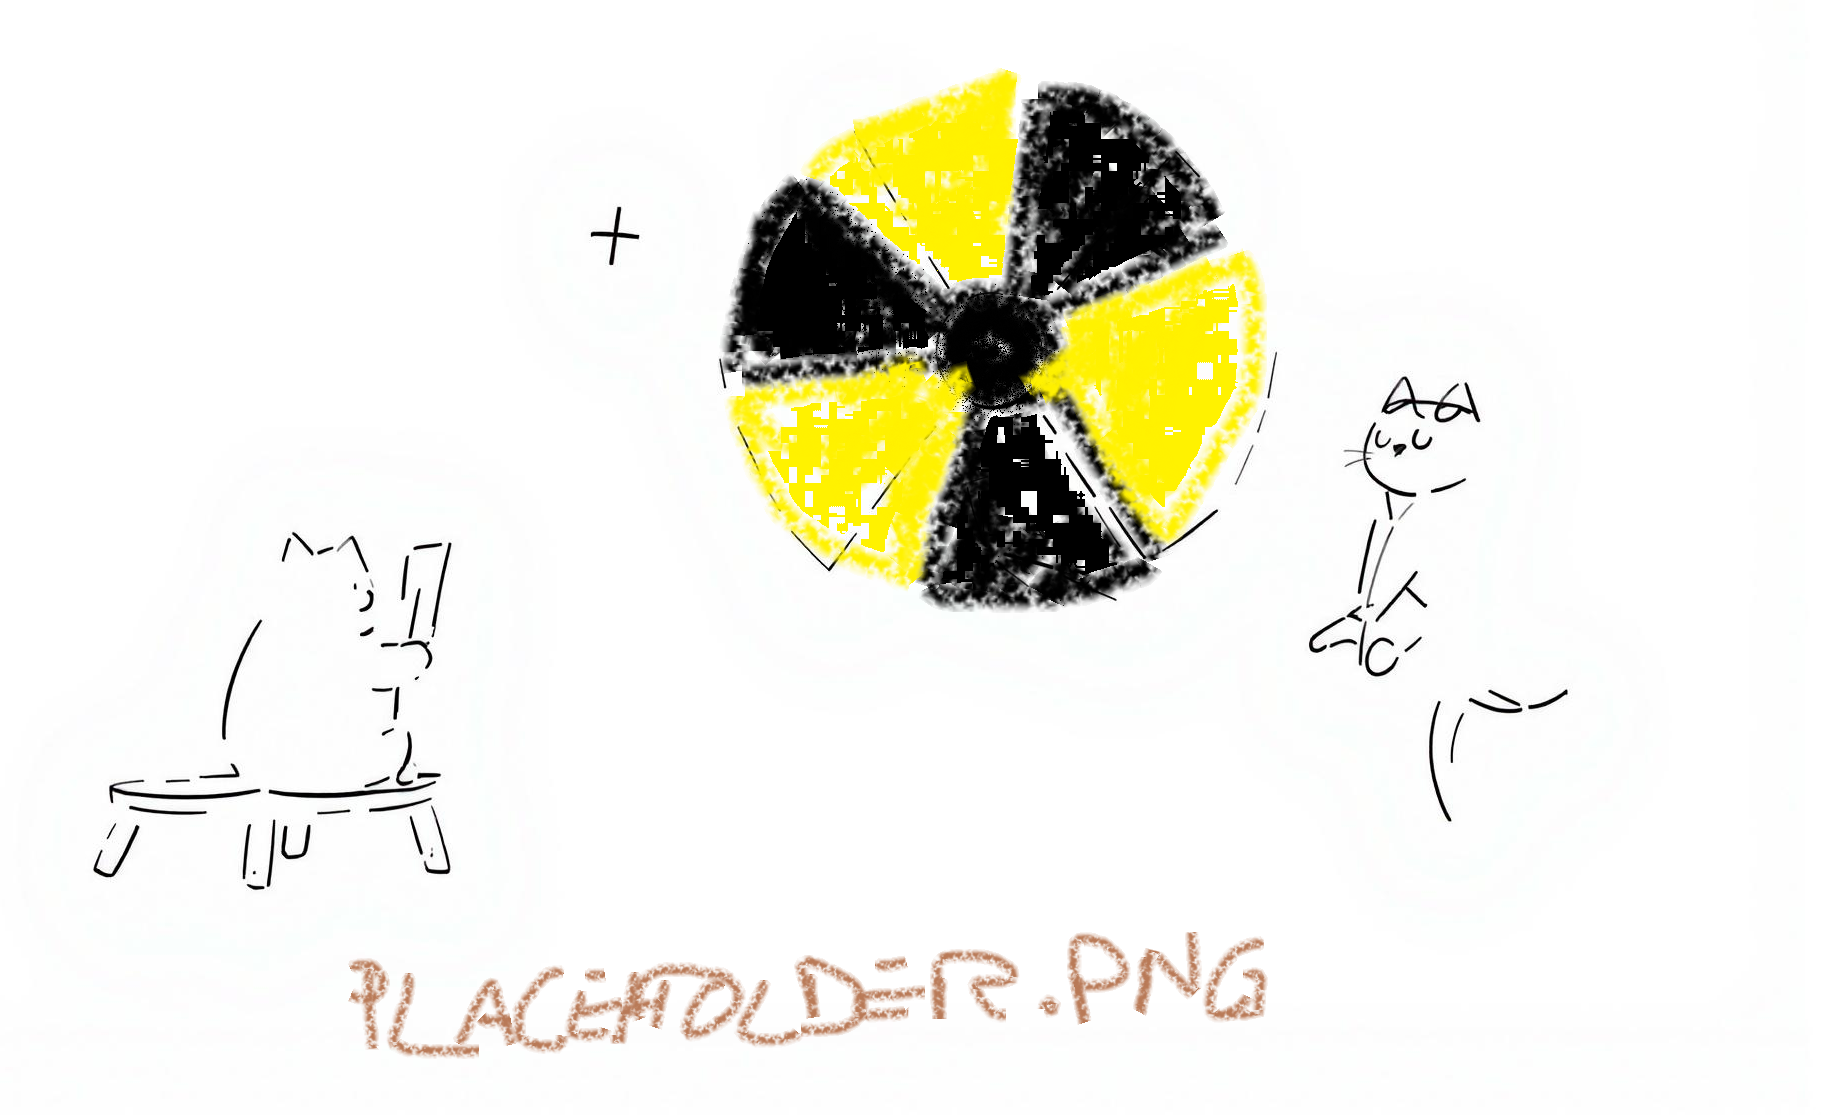
\includegraphics[width=\textwidth]{figures/placeholder.png}
        \caption{Local Net Electricity and Fossil Demand evolution over time.}
        \label{fig:net_electricity_demand}
    \end{minipage}
\end{figure}

The plots highlight several significant trends, including:
\begin{itemize}
    \item ...
    \item ...
    \item ...
\end{itemize}


\subsubsection{Water Usage}
The impact on water resources, primarily required for reactor and Balance of Plant (BoP) operation as well as for the High Temperature Steam Electrolyzer (HTSE) units, is deemed negligible. This is due to the plant's location near Lake Maggiore—one of Italy's largest lakes—which ensures a stable water supply without significant disruption to the basin's hydrological balance or ecosystem.

\subsubsection{Land Use}
One of the key advantages of the proposed project is its minimal land use impact. The compact scale of the facility, combined with its placement in an area already approved for nuclear activities, ensures efficient use of space. The site is located within the Joint Research Centre (JRC) complex, which already hosts research reactors (ESSOR and Ispra-1) and associated nuclear infrastructure. Notably, a containment building is available on-site and is deemed suitable to house at least one of the two planned Small Modular Reactors (SMRs), greatly reducing the need for new construction and environmental disturbance.

\section{Possible Improvements}
\subsection{On the Data Collection}
If the data for each class were obtained from a set of real buildings in the region instead of just one, it would yield better results. Ideally, a statistically significant set of buildings and variable utilization profile could be used. Moreover, it would be beneficial to weigh the simulation data on the real energy requirements of those buildings. This is a much more complex task since it would require extensive data acquisition throughout the year.

From the simulation, humidification and dehumidification electricity needs are neglected since these plants are rarely installed today. A better evaluation would consider the possible future share of air treatment plants in the residential sector. For the purpose of this study, the share of installed air conditioning systems for cooling was assumed constant throughout the years, but it might increase in the future.

\subsubsection{Renewable Energy Sources}
Solar-thermal systems were neglected since they are considered not very impactful and complex to evaluate.

\subsubsection{Conversion to Primary Energy}
Time-dependent efficiency for heat pumps, taking into account the ambient temperature could improve the model.

\subsubsection{Other Electricity Demand}
This is the most complex contribution to evaluate, especially considering that it is not easy to forecast how electricity consumption will evolve in 60 years. Collecting a statistically significant number of data from the region regarding the type of appliances installed and their consumption would improve the simulation.
For the purpose of this study the appliances demand was assumed constant throughout the years.

\subsection{On the Plant Modelling and Simulation}
The Modelica model could be utilized to analyze the dynamic response of the plant to transient conditions, thereby evaluating the system's adequacy and frequency control capabilities. This analysis could focus on critical periods, such as specific days of the year characterized by significant demand oscillations.

Additionally, buffers with limited capacity could be modeled to further understand their impact on system dynamics. The hydrogen plant could be simulated to partially shut down some HTSE units, allowing for better adaptation to demand variations.

Incorporating chemical kinetics into the methanation model could enhance the simulation of the plant's dynamic response to transient conditions. Furthermore, the optimization of hydrogen tapped for market consumption could be based on a detailed analysis of the transportation sector.

Lastly, the sizing of the entire plant should be optimized based on a comprehensive economic assessment.

\subsection{On the Economic Study}

\section{Conclusion}
\section{Limitations and Possible Improvements}
\subsection{Data Collection}
If the data for each class were obtained from a set of real buildings in the region instead of just one, it would yield better results. Ideally, a statistically significant set of buildings and variable utilization profile could be used. Moreover, it would be beneficial to weigh the simulation data on the real energy requirements of those buildings. This is a much more complex task since it would require extensive data acquisition throughout the year.

From the simulation, humidification and dehumidification electricity needs are neglected since these plants are rarely installed today. A better evaluation would consider the possible future share of air treatment plants in the residential sector. For the purpose of this study, the share of installed air conditioning systems for cooling was assumed constant throughout the years, but it might increase in the future.

Regarding the renewable energy sources, solar-thermal systems were neglected since they are considered not very impactful and complex to evaluate.

Time-dependent efficiency for heat pumps should be accounted for, taking into account the ambient temperature could improve the model.

Assessing appliances electricity demand is the most complex contribution to evaluate, especially considering that it is not easy to forecast how electricity consumption will evolve in 60 years. Collecting a statistically significant number of data from the region regarding the type of appliances installed and their consumption would improve the simulation.
For the purpose of this study the appliances demand was assumed constant throughout the years.

\subsection{Plant Modelling and Simulation}
The Modelica model could be utilized to analyze the dynamic response of the plant to transient conditions, thereby evaluating the system's adequacy and frequency control capabilities. This analysis could focus on critical periods, such as specific days of the year characterized by significant demand oscillations.

Additionally, buffers with limited capacity could be modeled to further understand their impact on system dynamics. The hydrogen plant could be simulated to partially shut down some HTSE units, allowing for better adaptation to demand variations.

Incorporating chemical kinetics into the methanation model could enhance the simulation of the plant's dynamic response to transient conditions. Furthermore, the optimization of hydrogen tapped for market consumption could be based on a detailed analysis of the transportation sector.

Lastly, the sizing of the entire plant should be optimized based on a comprehensive economic assessment.

\subsection{Economic Assessment}


\subsection{Environmental Impact Assessment}
The impact on water resources — primarily needed for reactor operations, Balance of Plant (BoP) systems, and HTSE units — is considered negligible. 
This is largely due to the plant's proximity to Lake Maggiore, Italy's second-largest lake, which provides a reliable and abundant water supply without significantly affecting the its
hydrological balance or ecosystem.

However, a quantitative assessment of the water balance is recommended to determine precise water consumption and discharge rates. This evaluation should also consider potential 
thermal impacts on the lake caused by plant operations. Given the lake's considerable size, such impacts are expected to be minimal, but detailed modeling is necessary for confirmation. 
The results should be compared with applicable regulatory standards for industrial water use.

For modeling purposes, the water required by the electrolysers is assumed to be unlimited, based on the lake's ample supply. Consequently, water costs are excluded from the HTSEs' 
operational expenditure (OPEX), influencing the overall economic analysis.



\section{Conclusions}

The project demonstrates that hybrid energy systems can significantly reduce carbon emissions in the studied area by fully eliminating fossil 
fuel use for electricity generation. Moreover, it lays the groundwork for further decarbonization of the transportation and heating sector.

The plant model confirms the technical feasibility of the proposed system, providing a detailed, hour-by-hour account of energy and material 
flows both within the plant boundaries and between the plant and the surrounding community.

The plant layout was, at first, roughly designed primarily around the operational requirements of the gas turbine. As a result, the number of High-Temperature 
Steam Electrolyzers (HTSEs) and Small Modular Reactors (SMRs) was determined based on this component constraints. 
The plant was accordingly oversized, in order to ensure sufficient syngas production to let the gas turbine operate at full capacity.

The ambitious decarbonization goals led to a substantial portion of the nuclear-generated electricity being allocated to 
low-profit decarbonization processes — such as hydrogen and methane production — rather than being sold directly to the grid.

A key finding of the economic analysis is that the high initial capital costs of the full hybrid system are unlikely to be recovered if all 
components are built simultaneously. However, a phased implementation strategy can mitigate these costs and ultimately generate positive returns.

To manage the financial burden and benefit from advancements in relevant technologies, the installation of the 
HTSE-Methanator-Gas Turbine complex is postponed until the 20th year of operation. 
In the first phase, the electricity from the SMRs is sold directly to the grid, generating more immediate and profitable returns 
to help offset nuclear capital expenditures.

This phased strategy mirrors the real-world approach of deploying SMRs incrementally to finance subsequent units. 
Moreover, this strategic choice demonstrates resilience with respect to the main financial parameters possibly affecting its economic viability.

When combined with the project's strong decarbonization potential and the elimination of foreign energy dependence, these results make 
the proposal a compelling opportunity for the Seven Lakes region and a strategic use of the JRC's nuclear infrastructure.

\newpage

% Appendix
\appendix
\section*{Appendix}
\addcontentsline{toc}{section}{Appendix}

% Example appendix content
\begin{lstlisting}[language=Modelica, caption= Methanation Reactor]
model MethanationReactor
  import      Modelica.Units.SI;
  import Modelica.Blocks.Interfaces.RealInput;
  import Modelica.Blocks.Interfaces.RealOutput;

  // Parameters
  parameter SI.Volume V = 0.01 "Reactor volume [m^3]";
  parameter SI.Temperature T = 573.15 "Reactor temperature [K]";
  parameter SI.Pressure p = 1e5 "Operating pressure [Pa]";
  parameter Real A = 1e10 "Pre-exponential factor [mol/(m^3.s)]";
  parameter Real Ea = 100000 "Activation energy [J/mol]";
  parameter Real conversionEfficiency = 0.80 "CO2+H2 conversion efficiency";

  // Inputs: molar flow rates [mol/s]
  RealInput n_H2_in "Inlet molar flow rate of H2"
  RealInput n_CO2_in "Inlet molar flow rate of CO2"

  // Outputs
  RealOutput PCI "Lower calorific value [MJ/kg]"
  RealOutput m_flow_rate "Total gas mass flow rate [kg/s] (CO2+CH4+H2)"

  // Constants
  constant Real R = 8.314 "Gas constant [J/mol.K]";
  constant Real M_CH4 = 16.0 "CH4 molar mass [g/mol]";
  constant Real M_CO2 = 44.0 "CO2 molar mass [g/mol]";
  constant Real M_H2  = 2.0  "H2 molar mass [g/mol]";
  constant Real LHV_CH4 = 50.0e6 "CH4 PCI [J/kg]";
  constant Real LHV_H2  = 120.0e6 "H2 PCI [J/kg]";
  constant Real UHV_CH4 = 55.4e6 "CH4 PCS [J/kg]";
  constant Real UHV_H2 = 141.8e6 "H2 PCS [J/kg]";

  // Internal variables
  Real n_CH4_out, n_H2_out, n_CO2_out;
  Real m_CH4_out, m_H2_out, m_CO2_out;

  // Temporary variable
  Real CH4_formed;

  RealOutput PCS "Upper calorific value [MJ/kg]"
algorithm 
  // Conversion based on limiting reagent
  CH4_formed := min(n_CO2_in, n_H2_in / 4) * conversionEfficiency;

  // Molar flows after conversion
  n_CH4_out := CH4_formed;
  n_H2_out  := max(n_H2_in - 4 * CH4_formed, 0);
  n_CO2_out := max(n_CO2_in - 1 * CH4_formed, 0);

  // Mass flows [kg/s]
  m_CH4_out := n_CH4_out * M_CH4 / 1000;
  m_H2_out  := n_H2_out  * M_H2  / 1000;
  m_CO2_out := n_CO2_out * M_CO2 / 1000;

  m_flow_rate := max(m_CH4_out + m_H2_out + m_CO2_out, 1e-6); // stabilized

  // Calorific value [MJ/kg]
  PCI := max((m_CH4_out*LHV_CH4 + m_H2_out*LHV_H2) / m_flow_rate, 0);
  PCS := max((m_CH4_out*UHV_CH4 + m_H2_out*UHV_H2) / m_flow_rate, 0);

end MethanationReactor;

\end{lstlisting}
\newpage
\begin{lstlisting}[language=Modelica, caption= Methanation Control Input]
  model MethanationControlInput
  import      Modelica.Units.SI;
  import Modelica.Blocks.Interfaces.RealInput;
  import Modelica.Blocks.Interfaces.RealOutput;

  // Parameters
  parameter Real stoichRatio = 4 "H2:CO2 molar ratio (default = 4 for stoichiometric)";
  parameter SI.Time T = 0 "Response time for control ramp [s]";

  // Constants
  constant Real M_H2 = 2.0 "H2 molar mass [g/mol]";

  // Inputs
  RealInput m_H2_in "H2 mass flow rate [kg/s]"

  // Outputs
  RealOutput n_H2_out "H2 molar flow rate [mol/s]"
  RealOutput n_CO2_out "CO2 molar flow rate [mol/s]"

  // Internal variables (target values)
  Real n_H2_target;
  Real n_CO2_target;

  // State variables for first-order delay
  Real n_H2_delayed(start=0);
  Real n_CO2_delayed(start=0);

equation 
  // Convert to molar flow
  n_H2_target = m_H2_in * 1000 / M_H2;
  n_CO2_target = n_H2_target / stoichRatio;

  if T > 0 then
    der(n_H2_delayed) = (n_H2_target - n_H2_delayed) / T;
    der(n_CO2_delayed) = (n_CO2_target - n_CO2_delayed) / T;
  else
    n_H2_delayed = n_H2_target;
    n_CO2_delayed = n_CO2_target;
  end if;

  // Outputs
  n_H2_out = n_H2_delayed;
  n_CO2_out = n_CO2_delayed;
end MethanationControlInput;
\
\end{lstlisting}
\newpage
\begin{lstlisting}[language=Modelica, caption= H2 Buffer]
  model H2_Buffer
  Modelica.Blocks.Interfaces.RealInput mass_flow_in
  Modelica.Blocks.Interfaces.RealOutput mass_flow_out
  parameter Real stock = 0;

  Real Content(start=0) "Amount of mass stored in the buffer";

equation 
    // Mass balance differential equation
  der(Content) = mass_flow_in - mass_flow_out;

  // Ensure mass_flow_out does not exceed the available content
  mass_flow_out = if Content > 0 then min((1-stock)*mass_flow_in, Content) else 0;

end H2_Buffer;
\end{lstlisting}

\begin{lstlisting}[language=Modelica, caption= CH4 Buffer]
  model CH4_Buffer
  Modelica.Blocks.Interfaces.RealInput mass_flow_in
  Modelica.Blocks.Interfaces.RealInput mass_flow_out
  Modelica.Blocks.Interfaces.RealInput mass_flow_to_grid

  Real Content(start=0) "Amount of mass stored in the buffer";

equation 
  // Mass balance differential equation
  der(Content) = mass_flow_in - mass_flow_out - mass_flow_to_grid;

end CH4_Buffer;
\end{lstlisting}

\newpage
\begin{lstlisting}[language=Modelica, caption= Control Room]
  model Control_Room
  import Modelica.Blocks.Types.Extrapolation;
  import Modelica.Blocks.Sources.CombiTimeTable;

  parameter Real n_HTSE = 8;
  parameter Real manualTable[:, :] = fill(0.0, 2, 5);
  parameter Real n_Reactors = 1;

  // Inputs
  Modelica.Blocks.Interfaces.RealInput P_nuc(start=100e6);
  Modelica.Blocks.Interfaces.RealInput P_turbine(start = 10e6);
  Modelica.Blocks.Interfaces.RealInput P_HTSE( start =1e6);

  // Outputs
  Modelica.Blocks.Interfaces.RealOutput setpoint_H2;
  Modelica.Blocks.Interfaces.RealOutput mflow_tapSteam;
  Modelica.Blocks.Interfaces.RealOutput turbine_load;
  Modelica.Blocks.Interfaces.RealOutput fossil_fuel_demand;

  // Variables
  Real Energy_Excess(start=0);
  Real tap_Setpoint(start=0);
  Real ramped_HTSE;
  Real ramped_turbogas;
  Real total_fossil_fuel_demand;
  Real Demand;

  // Load CSV data
  CombiTimeTable loadProfile(
  tableOnFile = false,
  table = manualTable,
  columns = {2,3,4,5},
  timeScale = 3600,
  tableName = "",
  extrapolation = Modelica.Blocks.Types.Extrapolation.HoldLastPoint)

equation 
  // Output assignments from table
  ramped_HTSE              = loadProfile.y[1];
  ramped_turbogas          = loadProfile.y[2];
  Demand                   = loadProfile.y[3];
  total_fossil_fuel_demand = loadProfile.y[4];


  // GUI-visible outputs
  setpoint_H2          = ramped_HTSE / 10;
  turbine_load         = ramped_turbogas;
  fossil_fuel_demand   = total_fossil_fuel_demand;
  tap_Setpoint         = 2 * setpoint_H2;
  mflow_tapSteam       = max(0.001, tap_Setpoint);

  // Energy balance
  Energy_Excess        = n_Reactors * P_nuc + P_turbine - P_HTSE * n_HTSE - Demand*1e6;

end Control_Room;

\end{lstlisting}

\newpage

% Bibliography
\printbibliography

\end{document}